%----------------------------------------------------------------------------------------
%	SECTION 2
%----------------------------------------------------------------------------------------

\section{Academic Performance}


\begin{figure}[htbp]
	\centering
	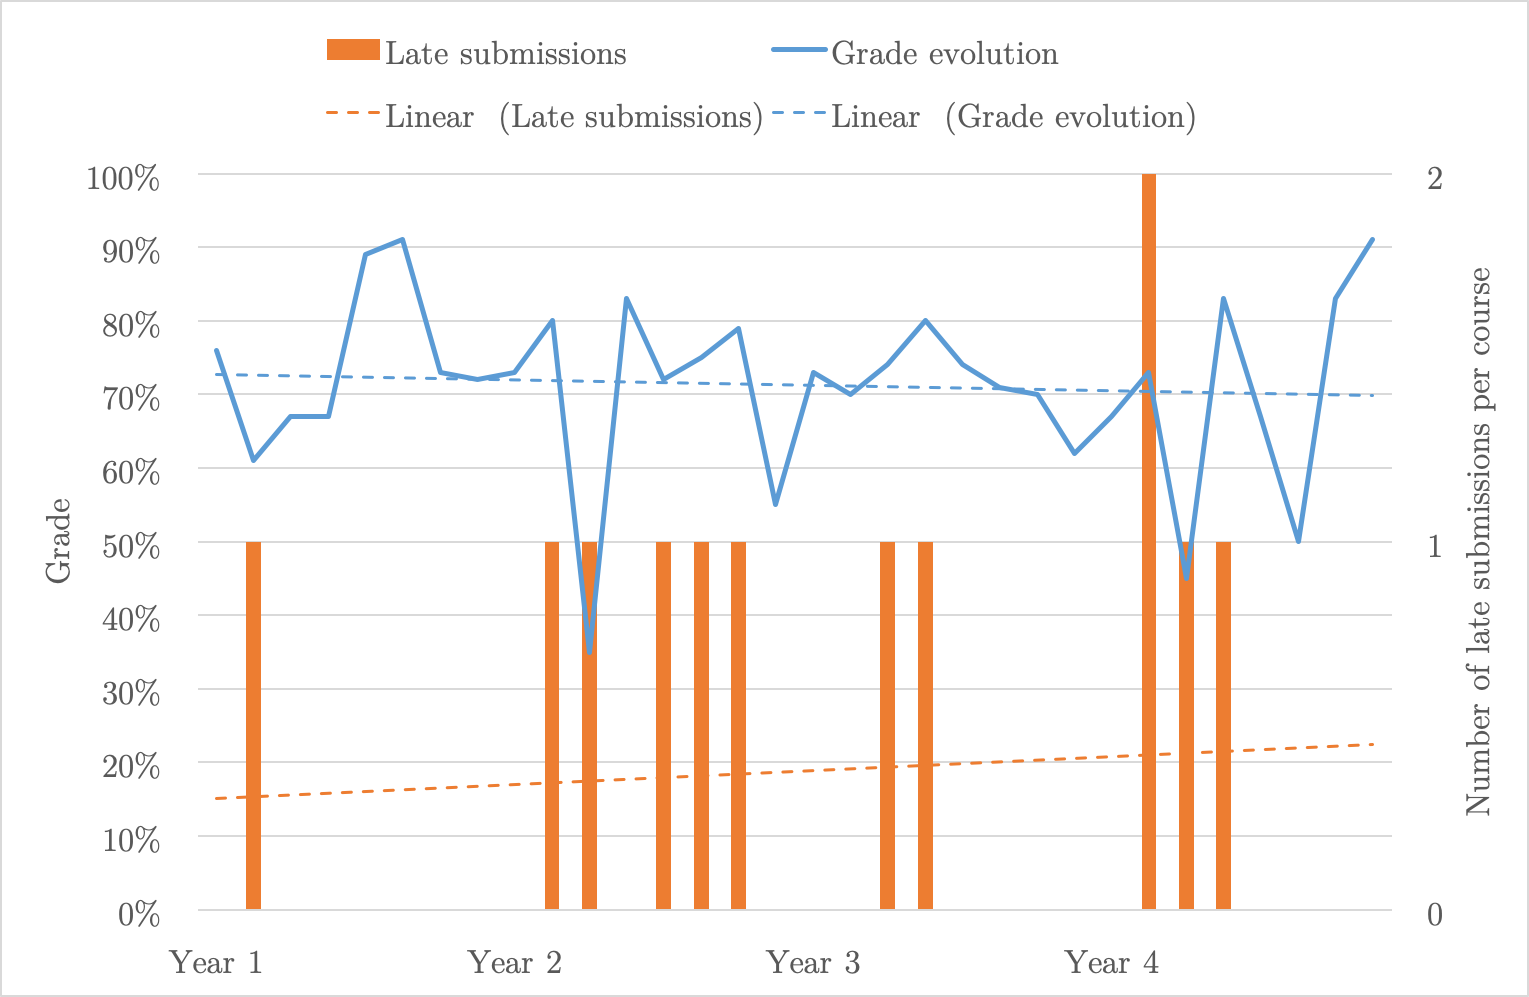
\includegraphics[width=0.9\textwidth]{figures/GradesVsLateSubs.png}
	\rule{0.9\textwidth}{0.5pt} % use line???
	\caption[Chart showing the evolution of my grades and late assignment submissions.]{Chart showing the evolution of my grades and late assignment submissions from Years~1 to 4 at Heriot-Watt University. N.B. Linear trendlines are represented by dashed lines.}
	\label{fig:gradesVlatesubs}
\end{figure}



%-----------------------
%   SUBSECTION 1
%-----------------------

\subsection{Meeting Deadlines}

%\hlc[green]{On reflection, I should have created the same Gantt chart (c.f. DST) to plan my work on this IP report. Now I feel like I have a whole lot to do and very little time.}



\subsubsection*{The Problem}

% SITUATION BEFORE UNI
I have struggled to meet deadlines for as long as I can remember.
Even in primary school, I once had to stay in during recess to complete an overdue piece of homework.
% (which I remember because I really wanted to go out and play with my friends).
In high school I thought I could overcome this problem by sleeping and exercising less.
This plan backfired as I found myself feeling moody, sluggish, and less productive.
Soon after that I started university and was again faced with deadlines.
This time I vowed to not deprive myself of sleep or exercise to meet my deadlines.
Instead I would prioritise these things, as I had learned that they contribute to my general well-being and productivity.
%So how was I going to manage my time better to submit assignments on time?

% SITUATION AT UNI
The problem continued at university.
The chart in Figure~\ref{fig:gradesVlatesubs} shows that there is a slightly increasing trend of my late submissions from Year 1 to 4.
%As the chart shows, I have not overcome my problem of submitting assignments past their deadlines.
Many of the late submissions are clustered in Year 2, when I submitted five assignments past their deadline.
Considering that I have taken 30 courses\footnote{This is the case if one merges both semesters of the \PRJTitle \space and \DSTTitle \space so that they become two courses as opposed to four.} 
over the course of my first four years at university, I have made late submissions for 11 of those courses, i.e. 37\% of all courses.
%However, one must consider that some of these courses were 100\% exam-based and the coursework for some others only consisted of giving presentations (for example) which cannot be submitted late.
%Hence, the percentage of late submissions would increase if one only considered the courses with relevant coursework.
During that time, the EGIS school-wide late submission penalty was a 10\% mark deduction if submitted within a week after the deadline; after the one week, a student gets zero marks for the assignment.
My average mark of the courses in which I made late submissions is 69\%, whereas that of the other courses is 73\%.
Thus, one can deduce that late submissions have had an overall negative effect on my grades.




\subsubsection*{Its Effect on Me}

Failing to meet deadlines has caused me some distress and damaged my confidence.
At one point, I did not believe I could make deadlines.
While my peers worried about meeting deadlines, I worried about making the week-after deadline.
Because of this, I put more pressure on myself to perform extra well on my assignments so that the 10\% penalty would not be as detrimental.

% CONCERNING PROBLEM
%In fact, it seems to be a growing problem which is 
The fact that I have not yet overcome this problem is concerning to me as I am about to start working in industry.
I do not want this problem to persist in my professional life as it could have more serious consequences than just a dent in my marks.




\subsubsection*{What I Learned From the Problem}


% CAUSE: TIME MGMT
%The root cause of my failure to submit assignments on time is poor time management.

% PROCRASTINATION
Often my approach to coursework has been to read around and prepare myself as best I can before starting the write-up.
This takes the form of extensive research and note-taking, in which I often organise and present my notes in various forms.
Now, those things are not necessarily bad to do, but because of the excessive amount of time I spent `preparing myself', these tasks eventually turned into forms of procrastination.
I would keep delaying the start of my write-up because I would not feel I have enough detail.
% DOUBLE WORK
Often, this method of working led me to do `double-work': for example, I might have written something by hand, but when it comes to the write-up on the computer, I essentially need to copy the handwritten notes.
If the notes were already in a digital format, I could have simply copied-and-pasted.
% DISADVANTAGE OF LATE SUBS

Another disadvantage I found with late submissions is their domino effect; if I have a series of deadlines, I have found that if I submit one assignment late, that it delays the submission of my other assignments, causing them to be late also.
This is reflected in the `clusters' of late submissions in Figure~\ref{fig:gradesVlatesubs}.

\begin{wrapfigure}{r}{0.5\textwidth}
	\centering
	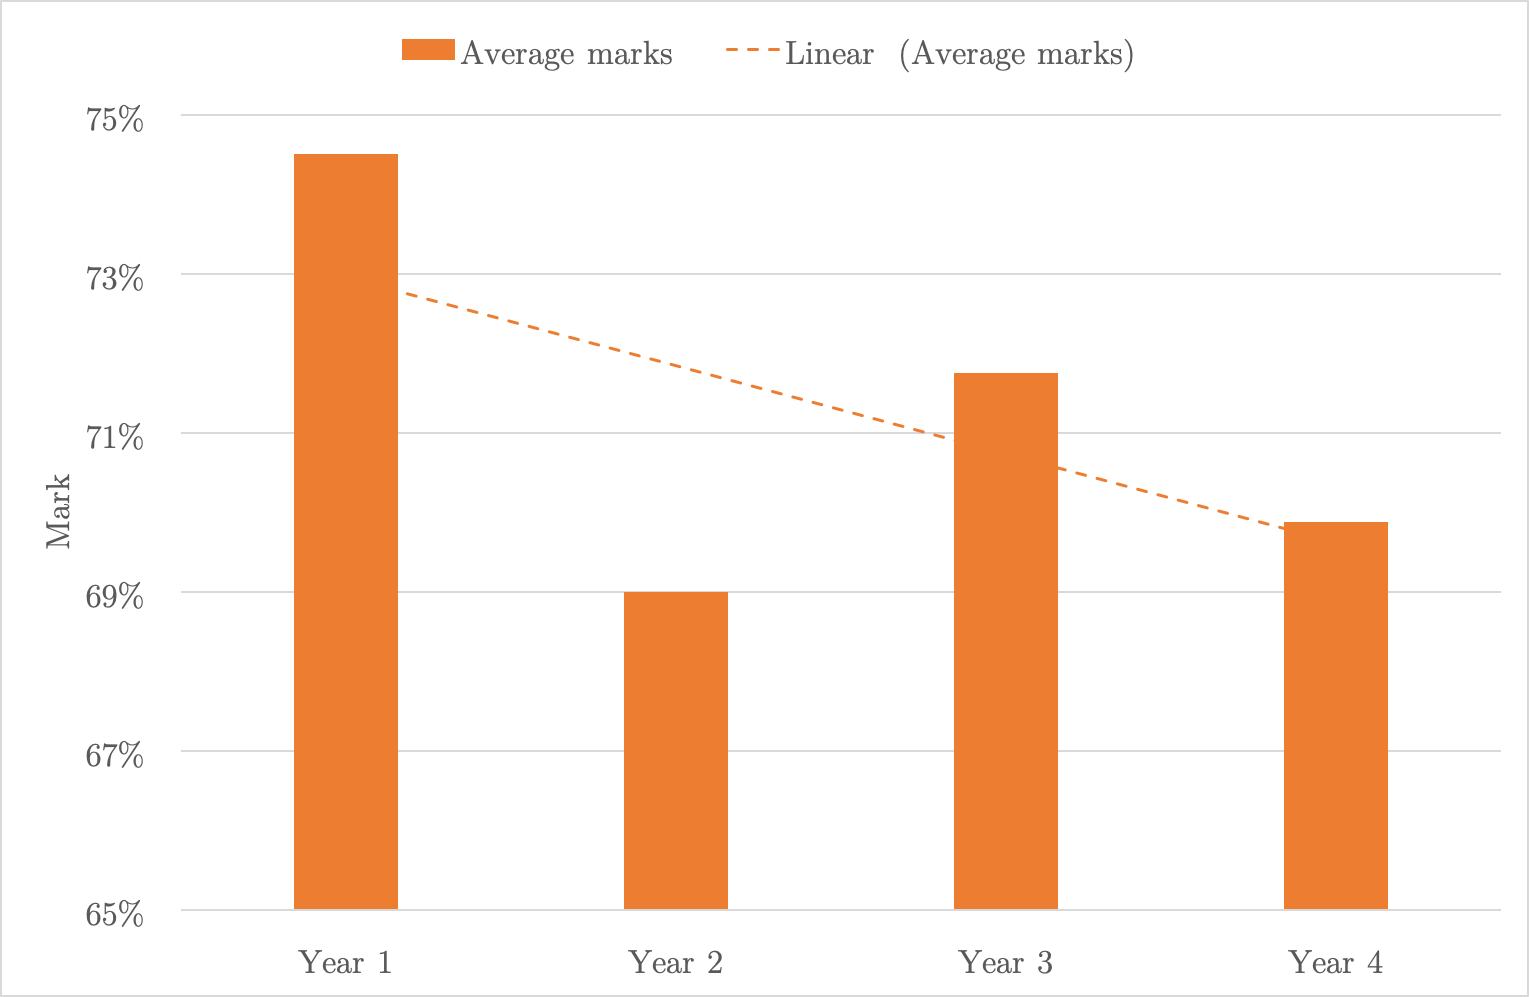
\includegraphics[width=0.5\textwidth]{figures/AverageMarks.png}
	\rule{0.5\textwidth}{0.5pt} % use line???
	\caption{My average marks from Years 1 to 4.}
	\label{fig:averages}
\end{wrapfigure}

% YEAR 2 DIFFICULTIES + WAKE-UP CALL + WHAT I LEARNED FROM YR 2
For most AE students, Year 4 is the most difficult.
For me, however, Year 2 was maybe as difficult as (if not more difficult than) Year 4.
This is reflected in my Year 2 average, which is the lowest average across the four years (see Figure~\ref{fig:averages}).
Looking at the trendline, one might have expected my Year 2 average to be the second highest.
I performed less well that year because there was coursework in every course, some of which were 100\% coursework-based, and I struggled to manage my time and all the assignments.
Other things that made Year 2 difficult were technically challenging and dense courses (especially \HYDTitle \space and \StatsTitle) and courses where one is required to work with uncertain or incomplete information (notably \textit{Design Projects A and B}).
The latter was revealed to me in my skills analysis in Section~\ref{sec:skills_ccl} as being linked to my perfectionist and risk-averse tendencies.
%I learned from my skills analysis in Chapter
%The work required for the design projects was unfamiliar; learning to navigate those courses with my risk-averse attitude was a challenge.
Failing \HYDTitle, largely because of a late submission, gave me the wake-up call I needed to address my time management problem.

% JUST INDIVIDUAL ASSIGNMENTS
%None of the late submissions are group assignments, all of %them are individual.
%I tend to prioritise group projects, because I do not want to ``let my group down".
%However, as a consequence, this has made me prioritise my individual assignments less.



\subsubsection*{What I Did to Improve}

% ATTEMPTS TO DEFEAT PROBLEM
I have made several attempts to overcome my problems of poor time management and failure to meet deadlines.
The following is a list of some of my successful and failed attempts.:
%Ways I have tried to do overcome my problem and their effects:

\begin{itemize}
	\item[$\times$] \textbf{Give up extra-curricular activities to gain time for coursework.}
	
	In Year 2, I gave up multiple activities/ responsibilities, including being on the Christian Union committee, being a class representative and playing volleyball.
	However, I have found that having more time does not necessarily equal getting more work done.
	It is essentially more time that needs managing.
	I was also reminded of my need for physical exercise, as I began to feel sluggish and unproductive again.
	I resumed exercising in Year 3.

	%\item[$\times$] \textbf{Not assign so much importance to an assignment.}

	%I found myself work on assignments worth 10\% or less with a lot more ease than large assignments.
	%With large assignments, there is an increased psychological pressure for me to do well, which makes it harder for me to actually start.
	%Unfortunately,
		
	\item[$\times$] \textbf{Divide up my time equally among my courses.}
	
	In Year 2, I performed below par on one of my four courses every semester.
	In Year 3, I noticed that I tended to neglect studying/ working on one of my four courses every semester.
	Having noticed this trend, I tried to divide up my time evenly per subject throughout the week.
	
	This turned out not to work so well.
	One of the reasons was because the work rhythms varied between the courses.
	Generally, if a course has coursework, its work tempo increases when an assignment has been announced, whereas a 100\% exam-based course may require regular study.
	Another reason this method did not work was because I found my workflow keep getting disrupted by switching from one subject to the other.
	From this I learned that I work better when I allocate large blocks of time (e.g. days) to focus on a single assignment/ subject.

	\item[\checkmark] \textbf{Start assignments as soon as they are announced.}
	
	This strategy was useful.
	After all, there is a reason professors allocate a certain amount of time for their students to complete assignments.
	However, this strategy needs to be accompanied by a `bird's eye' view, where the entire period allocated for an assignment is planned out.
	Otherwise, I found that I can fall into the same trap of stretching the time that I `prepare myself' for an assignment, thus leading to a late submission.
	
	\item[\checkmark] \textbf{Plan and monitor the entire work process.}
	
	I did this for the second stage of the \DSTTitle \space (see Figure~\ref{DST_schedule}) and found it very helpful to have an overview of the entire work process.
	It opened up my `tunnel vision' and enabled me to set time limits to different aspects of the work.
	Without these time limits, I would work on single aspects for unreasonable lengths of time.
	The schedule helped me submit my dissertation on time.
	
	%\item[\checkmark] \textbf{Avoiding double-work. Keep? If not, remove earlier mention of double work?}
	
	%by writing my notes out in a finalised format or document.
	%C.f. POSTnote	
\end{itemize}




\subsubsection*{Future Attempts to Improve}

Unfortunately, poor time management and failing to meet deadlines are ongoing problems.
Looking forward, I will try to implement the aforementioned lessons while maintaining a work-life balance.
In particular, I will try to take the time to plan and monitor the entire work process of an assignment to ensure I am working within the time limits.
This method, however, might still be restricted in that it only considers a single assignment, whereas I might have multiple assignments.
Therefore, next time I will try to create a programme which oversees and coordinates the work processes of all simultaneous assignments.


%-----------------------
%   SUBSECTION 2
%-----------------------

